\documentclass[10pt, a4paper]{article}
\usepackage{triada}

\graphicspath{{eps/}{png/}}

\renewcommand{\ell}{\mathcal{E}}

\usepackage{delim}
\usepackage{float}
\usepackage{subfigure}

                           
\begin{document}
\thispagestyle{empty}

\begin{center}
\ \vspace{-3cm}


\includegraphics[width=0.5\textwidth]{msu.eps}\\
{\scshape Московский государственный университет имени М.~В.~Ломоносова}\\
Факультет вычислительной математики и кибернетики\\
Кафедра системного анализа



%\vspace{5cm}
\vfill
{\LARGE Лабораторная работа}

\vspace{1cm}

{\huge\bfseries <<Анализ структуры потребительского спроса с помощью обобщённого непараметрического метода>>}
\end{center}

\vspace{2cm}

\begin{flushright}
  \large
  \textit{Студент 415 группы}\\
  Д.~И.~Степенский

  \vspace{5mm}

  \textit{Руководитель практикума}\\
  к.\,ф.-м.\,н., асс. А.~В.~Рудева
\end{flushright}

\vfill

\begin{center}
Москва, 2012
\end{center}

\newpage

\tableofcontents

\newpage

\section{Постановка задачи}
Требуется разбить товары на три интегрируемые группы, построить графики экономических индексов для каждой группы и для двух элементов каждой группы, а также построить и сравнить индексы Ласпейреса и Пааше и сделать вывод об использовании индекса построенного непараметрическим методом.

\section{Поиск интегрируемых групп}
Воспользуемся программным средством <<Система Индекс>> для выполнения поставленной задачи. За основу возьмем данные по товарам Венгрии, приложенные системе. Изменяя параметр рациональности поведения агентов $\omega$ ($\omega = 0$ означает рациональное поведение), получим различное количество интегрируемых групп:
\begin{itemize}
\item $\omega=0$: две группы (продовольственные товары; напитки);
\item $\omega=5\cdot 10^{-5}$: три группы (продовольственные товары; напитки; табачные изделия);
\item $\omega=10^{-4}$: пять групп (продовольственные товары; напитки; табачные изделия; образование, культура, спорт, отдых; прочие статьи потребления);
\item $\omega=2\cdot 10^{-4}$: шесть групп (продовольственные товары; напитки; табачные изделия; здравоохранение, гигиена; образование, культура, спорт, отдых; прочие статьи потребления);
\end{itemize}

Далее рассмотрим три первые выделившиеся интегрируемые группы: продовольственные товары, напитки, табачные изделия. Выберем из них по два представителя, соответственно: говядина и телятина, птица; вино, бренди; сигареты, табак. Построим графики индексов этих элементов, а так же графики индексов Пааше, Ласпейреса и индекса, полученного обобщенным непараметрическим методом.

\newpage
\section{Графики индексов. Сравнение}

\begin{figure}[H]
\centering\subfigure{
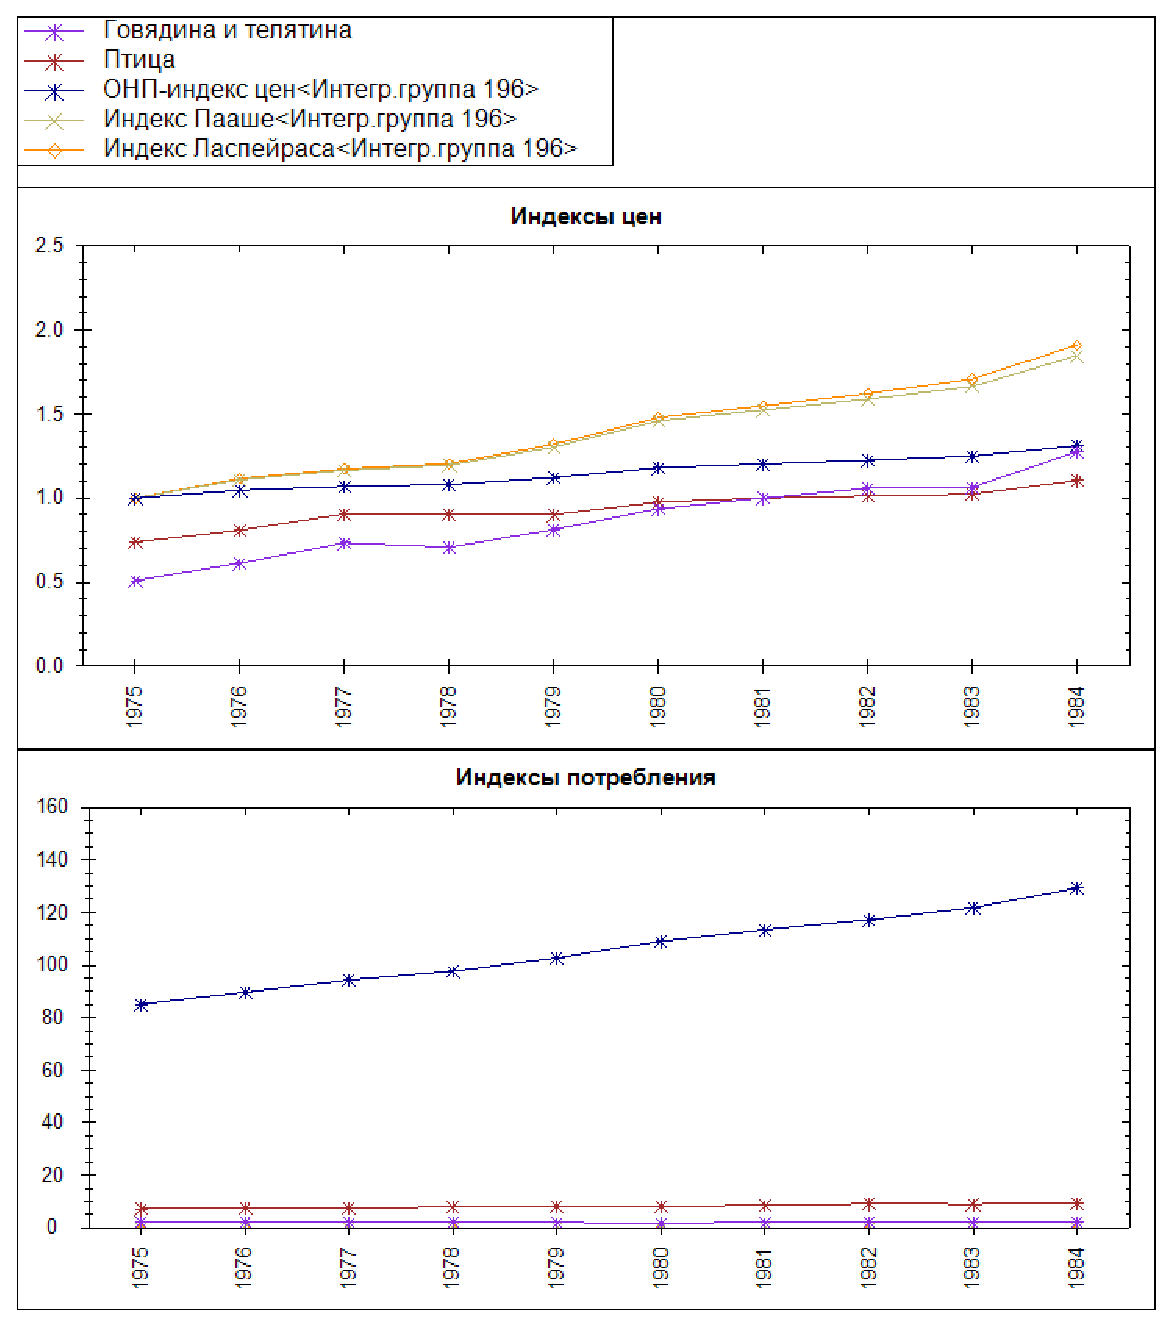
\includegraphics[scale=0.8]{prod.eps}
}
\caption{Графики для продовольственной группы.}
\end{figure}

\begin{figure}[H]
\centering\subfigure{
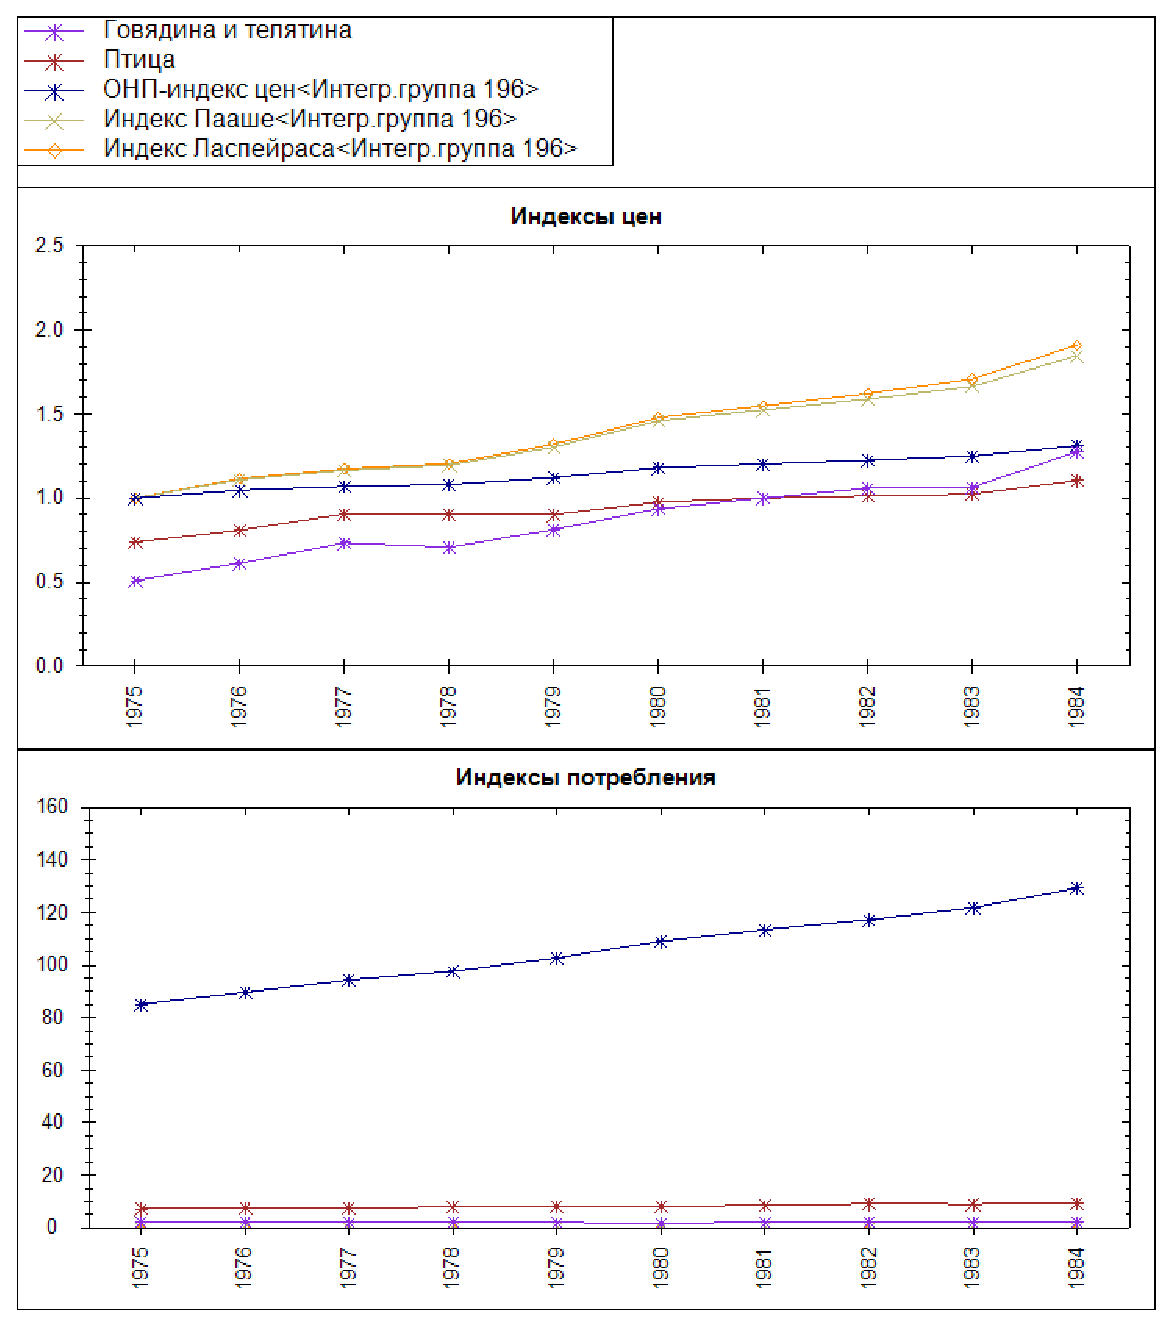
\includegraphics[scale=0.8]{prod.eps}
}
\caption{Графики для группы напитков.}
\end{figure}

\begin{figure}[H]
\centering\subfigure{
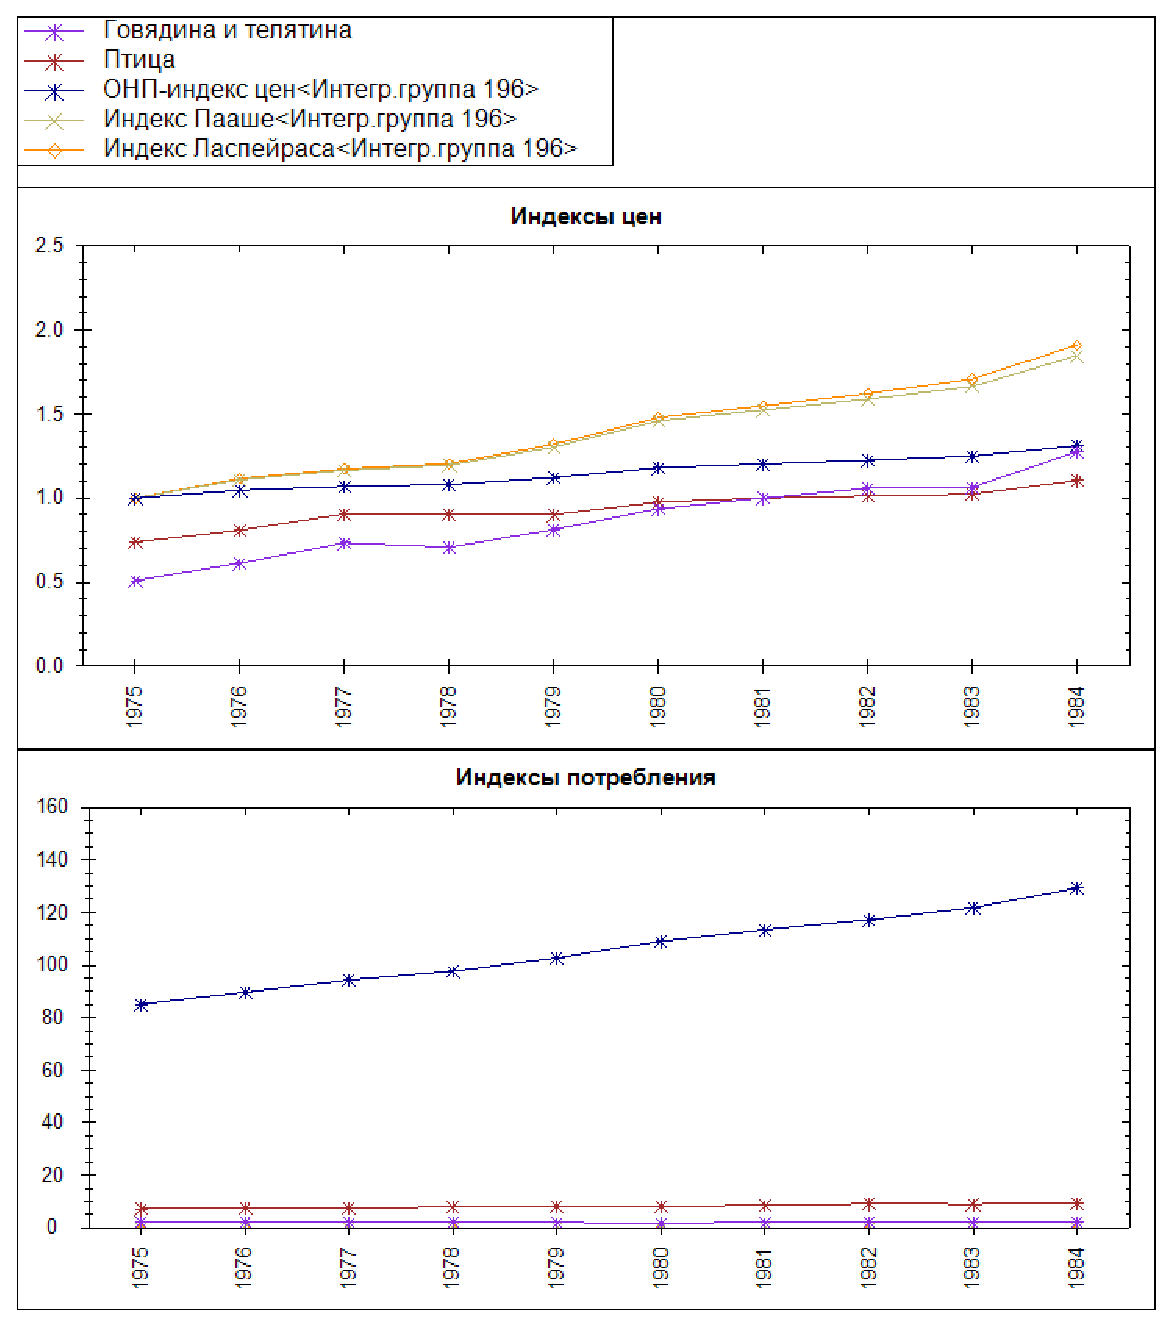
\includegraphics[scale=0.8]{prod.eps}
}
\caption{Графики для группы табачных изделий.}
\end{figure}

Как и доказывалось в курсе, индекс Ласпейреса оказался выше индекса Пааше. Кроме этого видно, что индексы Ласпейреса и Пааше более восприимчивы к изменению потребления товаров, чем индекс, полученный методом ОНП, однако менее восприимчивы к изменению цен конкретных элементов группы. 

\end{document}